\subsection{E5 -- Dedicated vs.\ shared user plane for URLLC}\label{sec:e5}
To test the design decision of \S\ref{sec:slices}, the URLLC probe (200\,Hz) ran under an
identical eMBB overload in two configurations. In \emph{dedicated} mode URLLC is anchored on
UPF-B. In \emph{shared} mode the SMF/UPF-A configs put the \code{urllc} DNN on UPF-A, the
same UPF as eMBB. To make the offered load identical in both modes, eMBB was a fixed-rate UDP
flood (2 UEs $\times$ 500\,Mbit/s downlink) with Session-AMBR and the tc MBR lifted. The
modes were alternated over three repetitions each, so that host drift affects both equally.
During the load phase the VM had no idle CPU. The iperf3 senders alone used about 3 of the 4
vCPUs, followed by \code{open5gs-upfd} (23--42\,\%) and \code{nr-gnb} (20--41\,\%). This is a
deliberately extreme stress test, not an operating point.

\begin{figure}[H]\centering
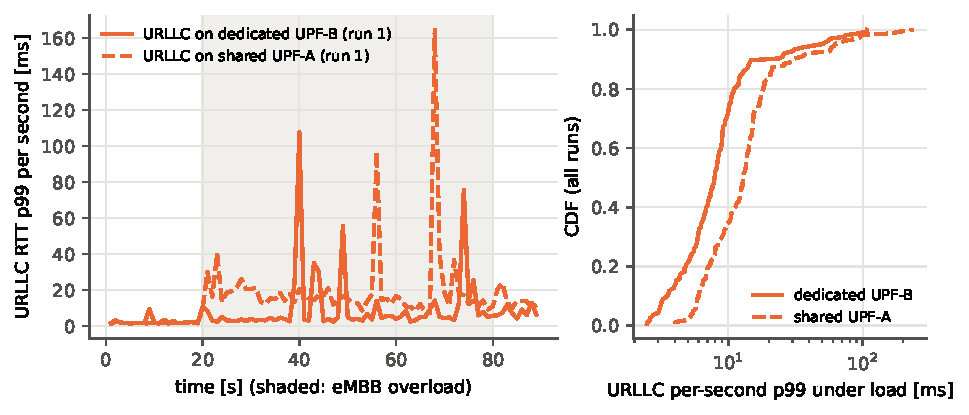
\includegraphics[width=0.86\linewidth]{figures/fig_e5_upf.pdf}
\caption{E5: URLLC per-second p99 RTT in the first run of each mode (left), and the CDF over
all three runs per mode (right, log scale). Shaded: eMBB overload.}\label{fig:e5}
\end{figure}

\begin{table}[H]\centering\small
\caption{E5 summary (mean $\pm$ s.d.\ over 3 runs per mode of the per-run median during load).}\label{tab:e5}
\resizebox{\linewidth}{!}{\begin{tabular}{lrrrrrrr}
\toprule
URLLC user plane & runs & load p50 [ms] & load p99 [ms] & p95 of p99 [ms] & worst p99 [ms] & loss [\%] & eMBB [Mbit/s] \\
\midrule
dedicated & 3 & 1.50 ± 0.86 & 7.42 ± 2.34 & 43.21 ± 9.97 & 107.5 & 11.937 & 58 \\
shared & 3 & 3.77 ± 1.90 & 11.78 ± 4.27 & 59.50 ± 22.36 & 237.4 & 4.831 & 41 \\
\bottomrule
\end{tabular}
}
\end{table}

Sharing the UPF made URLLC latency worse (Fig.~\ref{fig:e5}, Table~\ref{tab:e5}). Pooled over
all load seconds, the median of the per-second p99 rose from 7.9\,ms (dedicated) to 12.9\,ms
(shared). The share of seconds meeting the 10\,ms p99 target fell from 72\,\% to 35\,\%
(Mann--Whitney $p<10^{-11}$; the per-second samples are autocorrelated, so this overstates
the significance). At the correct statistical unit (one value per run, $n$\,=\,3 per mode),
the shared configuration has a 2.5$\times$ higher median RTT and a 1.6$\times$ higher p99, but
Welch's test gives $p$\,=\,0.16 and 0.22. The direction is consistent in two of three
pairs, but more repetitions would be needed to claim significance. URLLC \emph{loss} was
substantial in both modes and, unexpectedly, higher with the dedicated UPF (11.9 vs.\
4.8\,\%). Packets are dropped in components that both modes share, the user-space gNB/UE
(RLS) and the starved CPU, which UPF separation cannot isolate.
